

\chapter{Preliminaries}\label{chapter:preliminaries}

\section{Cyber-Physical Systems}

"Ubiquitous computing"

\begin{itemize}
\item characterized by limited resources
\item often real-time systems
\item often safety critical
\item Sensors and actors connected to ECUs
\item Examples of a cyber-physical system are vehicles
\item x-by-wire
\end{itemize}


\paragraph{Automotive System Engineering}
Control systems in modern vehicles are typically implemented as a collection of dozens, if not hundreds, of Electronic Control Units (ECUs) dispersed within a vehicle. Originally, there was no conscious decision to design automotive systems that way. Much rather, it is the result of an evolutionary process. At first, individual ECUs, each dedicated to a single purpose, were implemented in vehicles. At this point, ECUs were isolated from each other and no sense of cohesion was present in the system. This changed with the introduction of advanced wiring and bus systems that allowed ECUs to interact with sensors and actors. It was then only a matter of time until the bus systems were used to furthermore interconnect ECUs, which could then be used in interplay to create new, innovative functions \cite{broy2006challenges}. However random this evolution might have been, there are several benefits to the dispersed approach (as opposed to a centralized one). By having ECUs close to the sensors and actors they control, wiring effort is kept low, which results in low transmission latencies. 

Problems according to \citeauthor*{broy2006challenges}:
\begin{itemize}
\item Often highly proprietary
\item Limited re usability of software: 90\% of software is re-written 
\item Lack of tools and automation
\end{itemize}


Industry profile according to \citeauthor*{broy2006challenges}:
\begin{itemize}
\item Highly modular: several teams working independently on different technologies
\item Much is outsourced: many technologies are developed by suppliers, rather than the OEM 
\item Development: Many systems must interact -> vehicles evolve from an assembled device to an integrated system
\item Behavior becomes programmable: from comfort functions to steering and breaking: everything can be controlled by software.
\item moving away from specialized ECUs to general-purpose commodity systems
\end{itemize}

%
%
%
%
%
%
%
%
%
%

\section{Distributed Systems}
Modern vehicular E/E-Architectures\footnote{Electric/Electronic} are comprised of a large number of distributed, connected sensors, actors and control units, and hence, fall into the category of \emph{distributed systems}. The term "distributed system" entails many things and just as many definitions of the term exist. A definition that most would agree upon is the one given by \citeauthor*{tanenbaum2017distributed} \cite{tanenbaum2017distributed}: 
\begin{quote}
"A distributed system is a collection of autonomous computing elements that appears to its users as a single coherent system."
\end{quote}

The first aspect to consider in this definition is the word \emph{collection}. Distributed systems are made up of a number of \emph{nodes} which may occur in the form of either hardware devices, or software processes. Nodes work together to achieve a common goal. For this, they need to exchange messages (\cf \autoref{sec:middlewares}). Furthermore, the definition names \emph{autonomy} as a characteristic of distributed systems. Nodes, on their own, are autonomously acting entities, with their own, individual sets of rules and behavior. At the same time the system needs to be kept together. \emph{Groups}, which individual nodes may join, are a tool to achieve this. There are open groups, which every node may join, and closed groups, which employ an authorization mechanism to control access. 
Groups aim to provide \emph{coherence}, which is another aspect of the definition given above. By the given definition, however, the coherence of the system is only \emph{perceived}. \Ie , to users, whether they are humans or programs, a distributed system presents itself as a single entity, even though it is in actuality comprised of a number of physically dispersed processes and resources. This principle is called \emph{distribution transparency}. \citeauthor*{tanenbaum2017distributed} \cite{tanenbaum2017distributed} separate this principle into several aspects. The first one to note is \textbf{location transparency}. At the root of location transparency is the desire to hide the physical location of resources. A common method to achieve this is through the assignment of names. A user who wants to access a resource can thus refer to it by name, \eg\ a URL\footnote{"Uniform Resource Locator"}, while remaining oblivious of its actual location. Under the hood, communication is still based on location-dependent addresses, but such details can be hidden by a name resolution service. Naming furthermore facilitates another kind of distribution transparency: \textbf{Relocation transparency}. As the name suggests, relocation transparency aims to hide the fact that resources may move without the user taking notice. In the example of the aforementioned name resolution service, this can be achieved by reconfiguring the service to redirect users to a location different than the one previously known. To the user, still, the resource appears to be in the same location as it only knows its name. Related to relocation transparency is \textbf{migration transparency}, but in contrast to the former, migration transparency refers to the mobility of the \emph{user}. A migration transparent system allows a user to roam freely, while maintaining connectivity to the rest of the system. Examples of such systems are cellular networks.

Another aspect of distribution transparency is \textbf{replication transparency}. Distributed systems often provide means to replicate nodes or resources, \eg\ to improve availability and scalability. Replication transparency states that all such replicas appear as one to the user. In addition to scalability, replication can be helpful to provide failure resilience. If a given node fails, and a replica is available, the user can be automatically redirected to the replica. This is also known as \textbf{failure transparency}.

Another way in which a distributed system can be transparent is in terms of concurrency. Resources are often times shared among a number of users which are concurrently using the system. A desirable trait thereby is to hide this fact from the user such that the they are lead to believe that they are the only one with access to that resource. This is called \textbf{concurrency transparency}.

The last kind of distribution transparency that \citeauthor*{tanenbaum2017distributed} define is \textbf{access transparency}. Access transparency refers to how data is presented to different users. Several users may have entirely different views of the same data\todo{explain better}. At the basis of this is a basic principle of software engineering: the separation of data and its representation.

%
%
%
%
%
%
%
%
%
%

\section{Middlewares} \label{sec:middlewares}
A prerequisite for the coherence property of distributed systems is the need for nodes to engage in collaboration. More precisely, distributed applications need a way to pass messages, or data, between different threads of execution. For this purpose, \emph{middlewares} \cite{bernstein1996middleware} are commonly used. Although message passing is a prime example of a middleware's use case, there are many other important concepts for which middlewares exist, \eg , transaction management in database systems. The primary goal of middlewares is to abstract away such concepts so that programmers can focus on implementing business logic and shipping features, instead of having to deal with the underlying specifics. Middlewares are implemented as a software layer that sits between operating system and the actual applications. They are often included in the form of libraries that make the middleware's functionality available to the programmers by means of an Application Programming Interface (API). 

The need for middlewares becomes particularly evident in the example of \emph{messaging}. Messages need to be sent over a physical mediums which are often, by nature, unreliable. To ensure reliability, many things need to be taken care of, \eg , error detection, repetition mechanisms, etc. In addition, guarantees must be given that messages are delivered to the right receivers. Therefore, addressing and routing mechanisms must be in place. These are just a few examples of hard-to-solve problems related to messaging. Managing these things manually, and implementing according measures from the ground up is hardly feasible for programmers. Messaging middlewares greatly ease this process. 

\begin{figure}[htpb]
  \begin{tabular}{c}
  \begin{lstlisting}[language=C++]
auto& middleware = MW::register_by_name("Alice");
middleware.broadcast("Hello, World!");
  \end{lstlisting}
  \end{tabular}
  \caption[Middleware send example]{An examplary code snippet demonstrating a broadcast dispatch via middleware}\label{fig:send}
\end{figure}

\begin{figure}[htpb]
  \begin{tabular}{c}
  \begin{lstlisting}[language=C++]
void receive(const std::string& message, const std::string& sender) 
{ 
  // message = "Hello, World!"
  // sender = "Alice"    
}
  \end{lstlisting}
  \end{tabular}
  \caption[Middleware receive example]{An examplary callback function to receive messages via middleware}\label{fig:receive}
\end{figure}

\autoref{fig:send} and \autoref{fig:receive} show code snippets demonstrating the sending and receiving capabilities of a hypothetical messaging middleware. In the example, all a programmer needs to do to send messages is to invoke a simple function, \eg , \texttt{sendBroadcast} in \autoref{fig:send}. The middleware then ensures that the message is delivered to the right recipients over whichever transport is available. To receive messages, the programmer may, in the case of this exemplary middleware, define a callback function which the middleware calls automatically whenever a new message is available. An example of such function is depicted in \autoref{fig:receive}. In the callback function's body, logic could be implemented to process the message content passed in the \texttt{message} parameter.

%
%
%
%
%
%
%
%
%
%

\section{Networking}

\subsection{Overlay Networks}
Distributed systems are often organized as \emph{overlay networks}\footnote{The term "overlay networks" is often used interchangeably with its abbreviated form, "overlays"} \cite{tarkoma2010overlay}. An overlay network is a logical network which connects nodes, or peers, in an abstract, high-level manner. Naturally, in order to enable information exchange between the peers, overlay networks require a substrate physical network (\emph{underlay}) over which data can be transmitted. As opposed to physical networks, which connect \emph{physical machines}, overlay networks connect \emph{processes}. An important thing to note is that overlays aim to be as decoupled as possible from their respective underlays, such that both networks may evolve (change topology) independently without affecting their operability \cite{tanenbaum2017distributed}. For example, an added node in an overlay network does not necessarily entail the addition of a physical node. Conversely, the removal of a physical node does not necessarily result in connection loss of a logical node. An example of this is the Internet \cite{vaezi2017virtualization}, which spans a worldwide network of nodes that is resilient to failures, such that, when a physical node breaks, a redundant path to the target node may be taken. Other examples of overlay networks are VPNs, Peer-to-peer (P2P) networks and voice over IP (VoIP) systems. A schematic example of an overlay network is depicted in \autoref{fig:overlay}. The overlay spans over an underlay network, which in turn consists of three sub-networks. These sub-networks could be, \eg , company's internal network, the Internet, and a network within a data center. 

\begin{figure}[htpb]
  \centering
  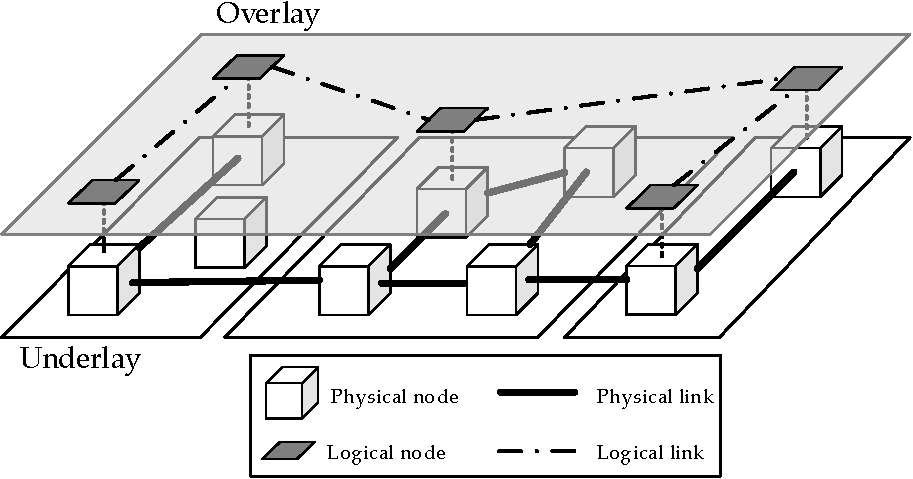
\includegraphics[width=0.8\textwidth]{figures/overlay.pdf}
  \caption[Overlay networking concept]{An overlay network on top of a physical underlay network which consists of three sub-networks}\label{fig:overlay}
\end{figure}

\citeauthor*{tarkoma2010overlay} defines two types of overlay networks: \emph{structured} and \emph{unstructured} ones. In the former, peers are organized in a specific, deterministic manner, such that each node has its firm place and an immutable set of neighbors. Unstructured overlay networks, on the other hand, allow the topology to change dynamically. In order for this to work, each node maintains an ad-hoc list of neighbors that is to be updated continuously \cite{tanenbaum2017distributed}. In the context of this thesis, unstructured overlay networks are of particular interest due to the dynamic nature and the reliability characteristics of mobile systems. 

\subsubsection{Virtual Local Area Networks}
\todo[inline]{Abschnitt unrund}
There are a number of ways to realize logical network overlays. VXLAN\footnote{"Virtual eXtensible Local Area Network"} and NVGRE\footnote{"Network Virtualization using Generic Routing Encapsulation"} two common examples. The technology used in the context of this work builds on VXLAN \cite{rfc7348}, an encapsulation protocol based on the long-established Virtual LAN (VLAN). VLANs make it possible to segregate a physical network into several isolated, logical networks. Each of those logical networks is assigned an identifier, a so-called \emph{VLAN tag}. All packets sent within a VLAN network have their respective network's VLAN tag attached on them at data link level (layer 2 in the OSI\footnote{"Open Systems Interconnect"} model). Based on the packet's tag, the substrate infrastructure can make decisions on how and where to forward packets. This allows for the realization of broadcast domains: each broadcast originating from a given VLAN network will stay within that network, regardless of how many other virtual networks exist alongside. This helps to significantly reduce network traffic.

Since the time when VLAN was devised much in the technological landscape has changed. In particular, virtualization has made great strides with the advent of cloud computing and multi-tenancy systems. Nowadays, thousands of virtual nodes dispersed throughout different clouds and on-premise infrastructures need to be connected. With its limited support for only 4096 virtual networks, VLAN cannot meet these increased demands. Thus, VXLAN was devised as a way to deal with the changed requirements. In contrast to VLAN, which is embedded in layer 2 protocol frames, VXLAN is an independent protocol which is placed on top of UDP connections (at application layer). In essence, VXLAN is a layer 2 overlay scheme on layer 3 networks, which effectively creates tunnels between Virtual Tunnel Endpoints (VTEPs). A VXLAN header contains a 24-bit network identifier which allows for the creation of 16 million virtual overlay networks. Encapsulated within each VXLAN frame is the actual packet sent from one application to another. Addressing in VXLAN is based on MAC\footnote{"Media Access Control"} addresses. In contrast to VLAN, these addresses don't necessarily have to be the actual hardware addresses of each host's respective NIC\footnote{"Network Interface Controller"}, but may just as well be virtual addresses of virtual machines. This makes it possible to address single VM instances within an overlay network individually, regardless of physical locality. 


\begin{itemize}
	\item provides layer 2 connectivity independent of physical locality and underlying network design
	\item VXLANs require software-based virtual network switches. Switching is moved to the data plane
\end{itemize}

\subsection{Multicast}
The simplest form of communication is one-to-one communication, which is also referred to as \emph{unicast}. In unicast, every node has an address by which it can be contacted. In most cases, unicast is sufficient for data exchange. However, in distributed systems, information frequently needs to be propagated to multiple receivers simultaneously. Unsurprisingly, this type of communication is called \emph{multicast} communication. 

benefits: No hard-coded addresses

Multicast can be implemented on both, network and application-level.

Support for multicast in WANs is rather limited.

\todo[inline]{TODO}

%
%
%
%
%
%
%
%
%
%

\section{Cloud Computing}

The idea of cloud computing is to provide access to remote computing resources  (\eg , networks, servers, storage, applications, and services) in a convenient, on-demand manner \cite{mell2011nist}. Customers of cloud providers can rent these resources to use them at their will. By outsourcing their IT infrastructure into the cloud, companies can significantly reduce capital and operational expenditures (CAPEX/OPEX) that are typically associated with running an on-premise infrastructure\todo{citation}. Other benefits include easier maintenance and accelerated time-to-market times\todo{citation, mehr benefits?}. Several pricing models for cloud services exist. Customers often have the choice between a set monthly fee, or they may take advantage of a pay-per-use model, whereby providers bill their users, \eg , on the basis of CPU time.

Cloud infrastructures are typically implemented as multi-tenancy systems in which the same hardware is shared among many customers. This principle is known as "resource pooling". An enabling technology for this is virtualization. Each customer is assigned one or more virtual machines (VMs) running on one or more physical servers. For its users, the alloted computing environment appears as a single, isolated physical machine. The amount of disposable resources can be controlled for each VM individually, allowing for fine-grained resource tuning according to demand.

A major selling point of cloud computing is scalability. Many cloud providers allow for the dynamic allocation of resources depending on demand. To customers, the available resources appear as if they were unlimited when in actuality the substrate resources are alloted and released under the hood in an elastic manner. To steer this behavior, \emph{elasticity controllers} can be employed which allow customers to define rules to control when and how scaling measures are performed. \Eg , when a CPU utilization threshold is reached, the system can be instructed to automatically launch an application replica. Subsequently, a load balancer can be used to distribute the load between the instances \cite{vaquero2011dynamically}.


\paragraph{}
Cloud computing presents itself in the form of several usage models. The most notable ones are: \emph{Infrastructure as a Service} (IaaS),  \emph{Platform as a Service} (PaaS), and \emph{Software as a Service} (SaaS) \cite{mell2011nist}, but many other models, mostly derivatives of the three mentioned, are in use today.

\begin{description}
\item[IaaS] In the IaaS model, sheer, usually virtualized, hardware is provided, on which customers can install and run arbitrary software. Customers have only basic control over their virtual infrastructure's hardware composition, but may take influence on the operating system level.
\item[PaaS] The PaaS model presents a higher level view on the infrastructure. In this model, customers don't have full control over their VM instance. Instead, they can deploy their software in predefined application-hosting environments \cite{mell2011nist} which are typically centered around a certain technology, \eg\ .NET, Node.js, etc. Examples for this type of services are Microsoft Azure or Google App Engine.
\item[SaaS] Finally, at the highest abstraction level of cloud usage models is the SaaS model\todo{sounds weird}. SaaS typically describes applications which are hosted on cloud platforms. These applications are usually accessible by means of thin clients, and most notably web browsers. Customers have the least control over the cloud service and can only take influence via application-level configurations \cite{mell2011nist}. Examples of SaaS applications are browser-based e-mail services or video streaming platforms.
\end{description}


\section{Linux Containers}

\begin{itemize}
	\item Why is there a need for virtualization?
\end{itemize}

In recent years, container technology has gained widespread adoption in the software development world. By greatly simplifying the software deployment— and development workflow, containers have become a cornerstone of successful software architectures.


Considering their advantages over hypervisor-based virtualization, such near native performance, sub-second boot times \cite{felter2015updated,morabito2015hypervisors} and minimal disk space usage, containers bring qualities to the table that are relevant specifically to embedded systems.

Containers are independent units of deployment containing everything a particular application needs to run from system libraries, tools, and runtimes to application specific settings. 
Akin to hypervisor-based virtualization, Linux containers aim to provide isolated, self-contained execution environments for applications that may be moved freely between hosts without affecting the application's behavior.
Unlike traditional virtual machines, however, applications in containers run on non-virtualized hardware, and thereby, with minimal performance overhead when properly configured \cite{felter2015updated,morabito2015hypervisors}. This is of interest particularly in the field of embedded systems where resource constraints are prevalent.

Enabled by a Linux kernel feature called \emph{kernel namespaces}, multiple containers may run on the same host side-by-side without affecting one another, or even having knowledge of each others existence. 
Namespaces wrap a set of system resources and present them to the container process as if they were dedicated to it. Each aspect of a container runs in its own namespace and its access is limited to that namespace. Through this, a decent level of isolation is achieved, albeit not as far-reaching as the isolation provided by VMs. The only thing containers share is the host's OS kernel, and optionally, parts of the file system.

In addition to providing isolation, containers employ resource management mechanisms which make it possible to allocate and limit the resources available to containerized processes. Resource management for containers is implemented by a kernel feature called \emph{control groups}, or \emph{cgroups} in short. Cgroups allow for the imposition of resource constraints (CPU-time, access to devices, memory budget, etc.) for groups of processes. Through this mechanism, containers, effectively \emph{being} groups of processes, can be restricted in what they can do and which resources they may take up. This opens up the possibility for container engines to exert fine-grained control over each container's resource utilization.

The two concepts (namespaces and cgroups) can be applied individually to any given process running on a Linux system. Only when combined together, such that processes are isolated through namespaces and restricted through cgroups, we speak of containers. In consideration of this it becomes clear that there is no clear distinction between a container and a process. Much rather, containers should be viewed as processes which are augmented by these two concepts.

%Further separation can be achieved through SELinux and AppArmor.

While it is possible to create containers manually utilizing the aforementioned native kernel features, such undertaking is rather cumbersome. For this reason, several tools are being developed which aim to streamline the use of containers. A few notable examples are \emph{\docker}\footnote{\url{www.docker.com}}, \emph{RKT}\footnote{\url{www.github.com/rkt/rkt}}, \emph{CRI-O}\footnote{\url{www.cri-o.io}}, \emph{Railcar}\footnote{\url{www.github.com/oracle/railcar}} and \emph{LXC}\footnote{\url{www.linuxcontainers.org}}. Among these,  \docker\ is undoubtedly the most prominent one, and arguably the first one to make Linux containers accessible for general use. For this reason, \docker\ was chosen for the approach presented in this thesis. Hence, the concepts described in the following are centered around \docker . 

\subsection{\docker\ Images}
Unique to \docker\ is its approach to container images. Images may be seen as the "blueprint" on the basis of which containers are built. Images are implemented utilizing UnionFS, a Linux service that facilitates the layering of different file systems atop each other. 
Leveraging this technology, \docker\ images are made of layers, with each layer adding to, or modifying, the respective underlying layer. 

Layers are immutable, such that, \eg , a file created in an underlying layer may not be deleted. Instead, when a change in the file system is performed, a copy-on-write layers is created, effectively adding another layer to the image.

A benefit of this approach is that individual layers may be shared and reused in other containers, thereby saving tremendous amounts of disk space compared to traditional VM images.

\subsection{\docker\ Engine}
The engine takes a container image and turns it into a container, \ie , a running process.

the engine can be controlled by means of a RESTful API. Most commonly, the engine is controlled by a command-line interface which makes calls to that API.

\subsection{Image Registries}

\subsection{\docker\ Networking}


% https://thenewstack.io/container-networking-breakdown-explanation-analysis/

\emph{libnetwork}

\docker\ provides several methods to create network links between containers.  



\paragraph{Bridge.} By default, \docker\ connects containers via a Linux bridge. Bridges are host-internal network interfaces. Through \texttt{iptables} functions like NAT\footnote{Network Address Translation} and port mapping are facilitated.

\paragraph{Host.} A Container in \emph{host} mode takes over the network interface of the host system. Therefore, all capabilities that that the host system possesses also apply to that container. A disadvantage of this is that only one container may run on a given host at any time.

\paragraph{Overlay.} 
Overlay networks \cite{tarkoma2010overlay} are ...
VXLAN as tunneling technology.
Serf as gossip protocol.
Implementations: flannel.
Benefits: Cross cloud connectivity, no public ports.

\paragraph{Underlay.}
MACvlan: Separate MAC and IP address assigned to each container. Eliminates the need for bridges and NAT, making it performant. Containers are entirely isolated from the host, increasing security.
IPvlan: Similar to MACvlan but instead of having one MAC address per container, all containers on a host share the same address. This works around a common security measure in network switches to prohibit the use of multiple MAC addresses per physical port.



\section{Data Distribution Service for Data Exchange}
Data Distribution Service (DDS) is a messaging middleware standard \cite{dds-1.4-standard} for distributed applications governed by the Object Management Group (OMG).\footnote{\url{www.omg.org}} DDS is designed for mission- and business critical systems with real-time requirements. As such, it aims to function in a resource efficient, predictable and reliable manner, and is subject to minimal computational and transport overhead.
Thus, DDS is a great fit for the automotive use case. 

\subsection{Data-Centric Publish-Subscribe}
DDS is fundamentally based on the data-centric publish-subscribe (DCPS) communication paradigm. In the publish-subscribe-style communication, data flows between two kinds of entities: publishers and subscribers. Publishers provide data, while subscribers consume that data. A crucial characteristic of publish-subscribe is that data exchange between the peers is anonymous, \ie , publishers have no way of sending data to individual subscribers. Instead, both communicate by means of a shared, logical medium that takes data samples and forwards them to the appropriate receivers. In the context of DDS, this medium is called \emph{topic}. When subscribers receive a data sample they do not know where that sample originated. Similarly, publishers have no knowledge about where the sent data will end up at---or even if there are any receivers at all. Entities in this system find each other not by way of addressing, but rather on the basis of a shared understanding of what \emph{kind of data} they want to exchange. This approach is called \emph{data centricity}. Data centricity is in contrast to \emph{message centricity}, in which data exchange is driven by \emph{messages}, or \emph{instructions}, which are directed at individual receivers. A prominent example of a message-centric technology is Remote Procedure Call (RPC). To illustrate the difference between the two paradigms consider the example of a temperature sensor (henceforth also ``provider'') which propagates temperature data to multiple receivers (henceforth ``consumers'').

\paragraph{Message-Centric Approach.} In the message-centric paradigm, the temperature sensor transmits data samples encapsulated in \emph{messages} to the consumers. Messages are directed at each consumer individually, similar to a letter that is addressed to a certain postal address. This requires each participant to maintain their peers' location information (\ie\ their addresses) in local memory.
Two patterns are common in message-centric communication: ``push-based'', and ``pull-based'' (often ``request-reply''-style) communication~\cite{tanenbaum2017distributed}.

If message-centric communication is push-based, the sensor needs to know the addresses of all interested consumers a-priori. The provider thus has to maintain a list of consumers that it needs to update continuously. When a previously uninvolved consumer decides that it wants to receive temperature data, it first needs to register to the sensor in order to make its address known. The sensor then has to add the consumer's address to its list of consumers. Similarly, when a consumer is shut down, the sensor needs to remove the respective address, and has to deal with unexpected errors in case a consumer is suddenly unreachable. This (un)registration procedure is the cause of overhead and additional management effort, and makes the system inflexible and hard to scale. In contrast, pull-based communication don't rely on lists of consumers, but consumers request information from the provider. In this regard, pull-based communication is more scalable, however, additional overhead is incurred since two messages (instead of one) need to be transmitted for each data sample: a request and a response. Furthermore, consumers can not predict when a new data sample is available. The situation is made worse when there is not one producer, but many. Thus, both approaches are highly inefficient in the use case at hand.

\paragraph{Data-Centric Approach.} The DCPS approach, on the other hand, is exclusively push-based.\footnote{Although request-reply-style communication is not explicitly supported it can be mimicked (\cf \Cref{sec:ddslatency}).} The temperature sensor is a publisher in the publish-subscribe relationship, and the consumers are subscribers. A subscriber that is interested in the sensor's data only knows that it wants to receive \emph{temperature data}, \ie\ data samples of type ``temperature'', and thus, subscribes to the ``temperature'' topic. 
The temperature topic is defined by a unique identifier and a data type. Only data of that specific type may be published on the topic. To ease the use of the middleware, DDS provides typed interfaces to the exchanged data. Through the optional \emph{Data Local Reconstruction Layer} (DLRL) \cite{dlrl-1.4-standard}, data types can be defined via the DDS IDL,\footnote{``Interface Description Language''} and according language-specific stubs can be generated. The use of type safe interfaces not only improves usability, but also increases safety and error-proneness, as verifications can be performed at compile time.

In the temperature sensor example, the subscriber is entirely oblivious to the concept of \emph{temperature sensors}, or even if there are any sensors---it just listens in on the ``temperature'' topic. Similarly, the temperature sensor is only concerned with the provisioning of temperature data, and doesn't know which subscribers to send the data to. Thus, the temperature sensor publishes all samples it gathers on the ``temperature'' topic. If more temperature sensors were to be introduced to the system, they could simply be added by registering new publishers which would post data on the same topic. Since all publishers of a topic identify themselves purely on the basis of their topic, and not by their address or location, a great deal of redundancy can be achieved---all publishers of a given topic are entirely interchangeable.
Due to the agnostic relationship between publishers and subscribers, a high level of loose coupling is achieved. This allows for a simple extension of the system, making it extraordinarily scalable.

It is often helpful to think of publish-subscribe communication not in terms of messages that are sent from one entity to another, but rather as a \emph{shared global data space} in which data is universally accessible to all entities involved in the system. In this data space, each entity views data as if it were available in a local storage, when in reality, it is distributed among many other entities.

\subsection{Under the Hood}
Naturally, in order to realize a publish-subscribe system, addresses and locations of nodes are still crucial, as publish-subscribe, like other communication paradigms, rely on IP-based computer networks. This fact, however, is hidden behind the curtains of the middleware (DDS in this case). The middleware is responsible for the registration of publishers/subscribers, the dissemination of data to the appropriate receivers, and the enforcement of network reliability policies. In order to do this efficiently, the middleware maintains lists of subscribers, publishers and topics. Many middlewares employ central components called ``brokers'' for this. Depending on the view point and use case, the centralized nature of brokers may be considered advantageous, or disadvantageous. On the one hand, centralization is associated with simplicity since everything is managed in one spot, and only one single source of truth exists. On the other hand, this approach brings the danger of a single point of failure that causes the whole system to fail if the broker fails. Additionally, centralized brokers may introduce bottlenecks, inhibiting the scalability of the system. 
As DDS is strongly focused on scalability, DDS employs a \emph{brokerless} architecture in which the functionality of the communication system is distributed among all participating entities. Consequently, message delivery as well as service discovery is performed in a decentralized manner.
For this, DDS may optionally employ IP multicast, by which all communication is directed at dedicated multicast group addresses, instead of each node's individual address. The delivery of data is then the responsibility of the underlying infrastructure.

\subsection{Wire Protocol}
DDS, in itself, is only a standard. As such, DDS does not dictate, in detail, how to implement the concepts presented in the earlier sections. A number of DDS implementations from different vendors exist, all varying in terms of standard compliance, features beyond the standard, licensing, and other distinguishing factors. Compatibility between the respective implementations can be achieved by the use of the DDSI-RTPS\footnote{The ``DDSI'' in DDSI-RTPS is often omitted. The shortened form will henceforth be used.} (DDS Interoperability--Real-Time Publish-Subscribe) wire protocol, which all major implementations support. Although the RTPS protocol is directly related to DDS, its specifics are outsourced in a separate standard \cite{rtps-2.2-standard}.
As a wire protocol, RTPS is deliberately tailored to DCPS-style communication. As such, it supports reliable multicast-enabled data exchange and service discovery over unreliable and connectionless best-effort transports such as UDP/IP. Special emphasis is put on robustness, fault tolerance, scalability and performance. Thus, RTPS was conceptualized with safety-critical real-time applications in mind. Although RTPS is the preferred transport method for DDS applications, it is not the only option. Many DDS vendors support TCP, UDP, and shared memory for cases in which performance is critical.

%
%
%
%
%
%
%
%
%
%
%
%
%
%
\subsection{DDS Components}
The DDS specification defines a number of components which are introduced in the following. \Cref{fig:dds} depicts an example highlighting how the components are related. In the example, there are two hardware nodes connected by an unspecified computer network. Each node can execute multiple applications simultaneously. The applications communicate with each other by means of DDS.


\begin{figure}[htpb]
  \centering
  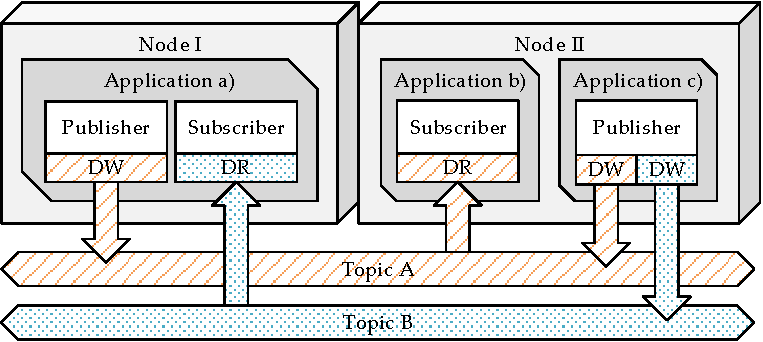
\includegraphics[width=0.8\textwidth]{figures/dds.pdf}
  \caption[An example of a distributed application connected via DDS]{An example of a distributed application connected via DDS}\label{fig:dds}
\end{figure}

\paragraph{Topics.}
\emph{Topics} form the basis on which peers communicate in the publish-subscribe paradigm. When a Publisher offers a certain kind of data, it does so by means of a Topic. When a data sample should be written, the Publisher pushes that data sample to a Topic appropriate for that sort of data. Conversely, when a Subscriber is interested in receiving data of a certain kind, then it subscribes to a Topic associated with that data. A Topic is uniquely defined by an identifier (name), a data type, and a set of QoS policies (see below). The data type represents the message format for data samples published on that Topic. For example, a suitable data type for a Topic concerned with temperature data would be a \texttt{struct} containing a single \texttt{float} value representing a temperature reading.
In \Cref{fig:dds} two Topics are depicted (Topic A and Topic B), each with a number of associated Data Writers and Data Readers (see below).

\paragraph{Publishers and Data Writers.}
\emph{Publishers} are entities that provide information in the publish-subscribe communication paradigm. Publishers are not bound to a single Topic. Instead, they contain one or more \emph{Data Writers}, each dedicated to a single Topic, who perform the actual data submission. Thus, Publishers may be seen as containers for a number of (unrelated) Data Writers. This concept is emphasized in \Cref{fig:dds} where a Publisher in Application c) controls two independent Data Writers that both write to different Topics.

\paragraph{Subscribers and Data Readers.}
\emph{Subscribers} are the exact compliment to Publishers in that they seek to receive data from Publishers. Analogous to Publishers, Subscribers are a way to group together sets of \emph{Data Readers}. Data Readers are entities whose purpose it is to receive data samples from their respective Topic. Through its API, DDS allows Data Writers to receive data in three ways: either by waiting for data samples (blocking the main thread), by pro-actively polling for new data samples, or by specifying asynchronous callbacks which are invoked whenever a data sample arrives.

\paragraph{Domains and Domain Participants.}
\emph{Domains} are the DDS way of grouping together sets of coherent \emph{Domain Participants} and to separate those sets from each other. Speaking in terms of distributed systems, Domains are a mechanism to manage group memberships of nodes \cite{tanenbaum2017distributed}. Domain Participants are entities that belong to a particular Domain. Each Publisher, Subscriber and Topic is derived from one Domain Participant and is therefore dedicated to exactly that Domain. As a consequence, participants of different Domains are entirely separated from each other and there is no way for them to interface with each other. Depicted in \Cref{fig:dds} is only one Domain. However, there could just as well be other Domains.
\pagebreak
\subsection{Quality of Service}
One of DDS's salient features is its intrinsic support for Quality of Service (QoS), which is realized by so-called ``QoS policies''. QoS policies specify attributes that can be used to control each component's behavior and quality properties. They make specifying a component's behavior a matter of \emph{configuration}, rather than \emph{implementation}. For example, consider a Data Writer which writes data to a Topic at a high rate. A Data Reader may be interested in that data but not at such a high rate, \eg\ because it runs on an embedded device powered by a battery and therefore needs to manage power consumption carefully. The Data Reader may now apply a \tbf , which instructs DDS to block all samples that exceed a specified frequency threshold. This way, the rate of incoming messages can be controlled via configuration. This is beneficial for the programmer as they do not need to accommodate for this at code level, but let the middleware take care of it.

QoS policies can be set for each Topic, Publisher, Subscriber, Data Writer and Data Reader individually.
In \Cref{tab:qos}, an excerpt of the available QoS policies is given. For the exhaustive list of all available QoS policies refer to the official standard \cite{dds-1.4-standard}.

Another example of a QoS policy is the \deadline\ policy. It specifies the minimum sampling frequency of a Data Writer. If the deadline period of a hypothetical Data Writer is set to, e.g., 100 ms, then this Data Writer is obligated to send a data sample at least every 100 ms. If it fails to send samples at this rate, the Data Writer and all the respective Topic's readers will be notified about that circumstance and are free to act accordingly.

In addition to specifying quality attributes, QoS policies may also serve as ``service contracts'' between interacting DDS components. These contracts specify non-functional requirements that the involved components must fulfill to be able to communicate with each other. For example, a Data Writer's \reliability\ policy may have been set to the \texttt{BEST\_EFFORT} level, thereby allowing the writer to drop samples. A Data Reader, on the other hand, may require the writer's policy to be set to \texttt{RELIABLE}, which prohibits the dropping of samples. Since the writer does not fulfill the reader's QoS requirements, the two components are considered incompatible, and thus, they cannot interact with each other.

Despite their name, QoS policies do not only concern \emph{quality} attributes per se. They can also be used to specify the priority of data samples, their lifespan, \ie , how long they are valid, or how many data samples of a certain type are kept in local memory.


\begin{table}[H]
  \caption[An excerpt of DDS QoS policies]{An excerpt of QoS policies}\label{tab:qos}
  \centering
  \begin{tabular}{p{0.25\textwidth} p{0.2\textwidth}  p{0.45\textwidth}}
    \toprule
      \textbf{Name} & \textbf{Legal values} & \textbf{Description} \\
    \midrule
    	\reliability  & \texttt{RELIABLE}, \texttt{BEST\_EFFORT} & Indicates whether a Data Writer may drop samples or whether a Data Reader approves of Data Writers that drop samples.\\
    	\tbf  & An integer value denoting time & Specifies a Data Reader's desired data reception rate. Superfluous samples will be discarded.\\
    	\liveliness  & An integer value denoting time & Defines the rules to determine whether a particular entity is ``alive'', \eg\ by emitting heart beats. \\
    	\deadline  & An integer value denoting time & Establishes a contract between Data Writer and Data Reader to determine the acceptable data rate. \\
    	\ownership  & \texttt{SHARED}, \texttt{EXCLUSIVE} & Specifies whether multiple Data Writers may write to a given Topic simultaneously or just the one with the highest \ostrength\  value.\\
    	\ostrength  & An integer value denoting relative priority & Determines a Data Writer's priority in cases where its Topic's \ownership\ is set to \texttt{EXCLUSIVE}. \\
    \bottomrule
  \end{tabular}
\end{table}
%
%
%
%
%
%
%
%
%
%
%
%
\pagebreak
\subsection{Redundancy and Automatic Failover} \label{sec:failover}
DDS has ways to ensure reliable communication---even over unreliable transmission channels. Part of reliability is failure transparency, \ie , the ability to quickly substitute failed components by backup components. The substitution process involves two steps: first, the failure needs to be detected. Second, a backup component needs to be instructed to take over. By means of the three QoS policies \ownership , \ostrength\ and \liveliness\ (\cf \Cref{tab:qos}), DDS may realize this process.

As the first step, a mechanism needs to determine whether a component has failed. In most cases, it is not possible for a failing component to properly shut down and ``sign off'', \ie , to notify the rest of the system that it will become unavailable. For this reason, the failure needs to be automatically registered. The \liveliness\ policy can be used to achieve this. \liveliness\ is the mechanism that determines whether a component is responsive (``alive''), or unresponsive (``dead''). The policy's value can be set to number indicating the maximum time interval between each liveliness signal. If a component fails to show a vital sign during that period, it is considered dead by the rest of the system. Passive components, \ie\ those which do not actively emit data, can be instructed to automatically send liveliness signals, or heartbeats, in certain intervals.

After a component has been declared dead it is up to the middleware to elect a substitute component. This is done through the \ownership\ and \ostrength\ QoS policies. By assigning a topic the \ownership\ value ``\qos{exclusive}'' one can specify that only a single data writer may write to that topic at any given time. Which data writer is given that prerogative is determined by the data writer's \ostrength\ value. The data writer that possesses the higher value is eligible to write to the topic. In the failover scenario, both, the primary data writer and the backup writer are assigned to the same topic, and both are configured to have exclusive \ownership\ rights. The former one has a higher \ostrength\ than the latter one. Based on both writer's \ostrength\ values, it is decided which one has precedence over the other.
%
%
%
%
%
%
%
%
%
%
%
%
%\subsection{Separation of User Data}
%The presented approach relies on a single cloud infrastructure, while at the same time, a vast number of customers need to be served. This poses a challenge concerning the separation of data. Confidentiality and privacy of user-specific application data must be preserved. Similarly, the result of a computation commissioned by a specific vehicle must be returned to exactly that vehicle, and no one else.

%Gladly, DDS offers a solution to this. In DDS, topics are not restricted to a single domain, \ie , they may be reused in multiple domains. If, \eg , a publisher belongs to \texttt{Domain $\alpha$} and publishes data on \texttt{Topic A}. Then, a data reader that reads from \texttt{Topic A} but belongs to \texttt{Domain $\beta$} may not read the data. Therefore, through domains, the same application may be reused several times on the same network, while keeping topic data separate. This principle is taken advantage of in the presented approach: domains are used to separate user data, such that for each user there is one user-specific domain. Thus, there is no way that data from one vehicle may interfere with data from another vehicle.

%\subsection{DDS for Automotive Systems}
%Automotive software systems have previously relied---and, to some degree, will continue to do so---on low-level, low-bandwidth transport protocols such as CAN, LIN, etc. For the longest time, networks stacks based on those protocols were sufficient to meet the basic requirements of delivering vehicular sensor data. However, driven by the emergence of innovative functions, the demands for vehicle intrinsic networks are skyrocketing. In particular, more and more sensor data from increasingly bandwidth-hungry sensors, such as cameras and lidars is feeding into advanced systems such as ADAS.
%At the same time, these functions require computational capabilities that go way beyond of what is possible with the microcontrollers typically used in traditional ECUs. High-performance computer systems based on high-level operating systems, supported by bandwidth-friendly networking protocols are needed to meet the new requirements.
%A new generation of low-level network protocols found their way into the vehicle. Notable mentions are FlexRay, and TSN. A question that remains is whether DDS is a suitable choice for the use within vehicles, and whether DDS may be used efficiently on top of these lower level protocols. \citeauthor*{bouhouch2013dds} have shown \cite{bouhouch2013dds} that DDS is indeed a suitable middleware to be used in vehicular networks.

%DDS allows to configure how much of a system's resources an DDS-enabled application may use. Consequently, it is the middleware's responsibility to allocate resources as needed while still staying within the specified boundaries. At the same time, priorities aligning with the application's QoS settings need to be considered. DDS takes this burden off the programmer's shoulders.
%\todo[inline]{TODO}


%
%
%
%
%
%
%
%
%
%
%
%
%
%
%
%
%
%
%
%




%
%
%
%
%
%
%
%
%
%

\section{Software Architectures}
\todo[inline]{move / remove}
\todo[inline]{
Today, there is a tendency for software architectures to shift away from the \emph{monolithic} paradigm of having a single software entity deployed on a single, potent server to a more \emph{distributed} paradigm where multiple components are spread over a number of less potent physical hosts connected over a network.
The benefits of this approach became evident in the early 2000's when a new type of software architecture utilizing this concept became popular: \emph{service-oriented architectures} (SOAs).

In recent years, SOAs have made a revival in the form of \emph{microservices}, which, in essence, is a more fine grained type of SOA that avoids the complexity induced by \emph{Enterprise-Service-Buses} (ESBs). Similar to SOA, the idea behind microservices is to split functionality into a collection of reusable components, each fulfilling a single specific purpose. Recent research efforts are evaluating the possibility to include such paradigm in the realm of automotive software systems -- in part achieving great success \cite{berger2017containerized}. 

Since Microservices are very limited in scope they may be built and deployed in a matter of minutes, rather than hours, as is the case with monolithic applications. Thus, microservices have the potential to tremendously accelerate the software development process when being combined with modern development practices such as \emph{continuous integration / continous delivery} (CI/CD).
}